\subsection{Size Measurements}
\label{appendix_size}

The images used to find $d_{hair}$ and $d_{gf}$ are presented in respectively figure \ref{fig_hair} and \ref{fig_gf}

\begin{figure}[h!]
    \centering
    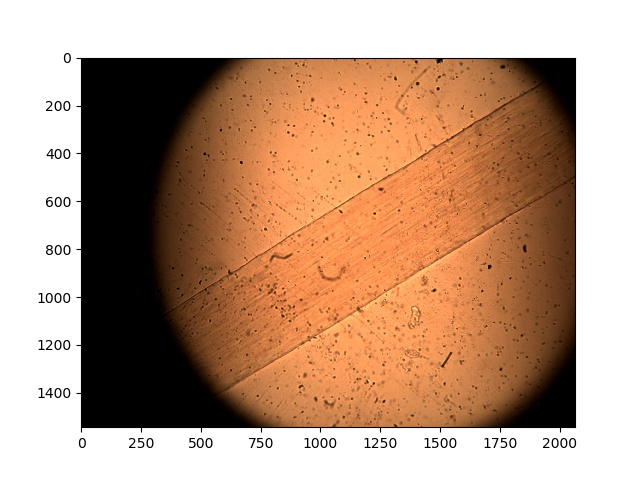
\includegraphics[width=7cm]{afbeeldingen/size/hair.jpg}
    \captionsetup{font=small, justification = centering}
    \caption{Image used to find $d_{hair}$.}
    \label{fig_hair}
\end{figure}

\begin{figure}[h!]
    \centering
    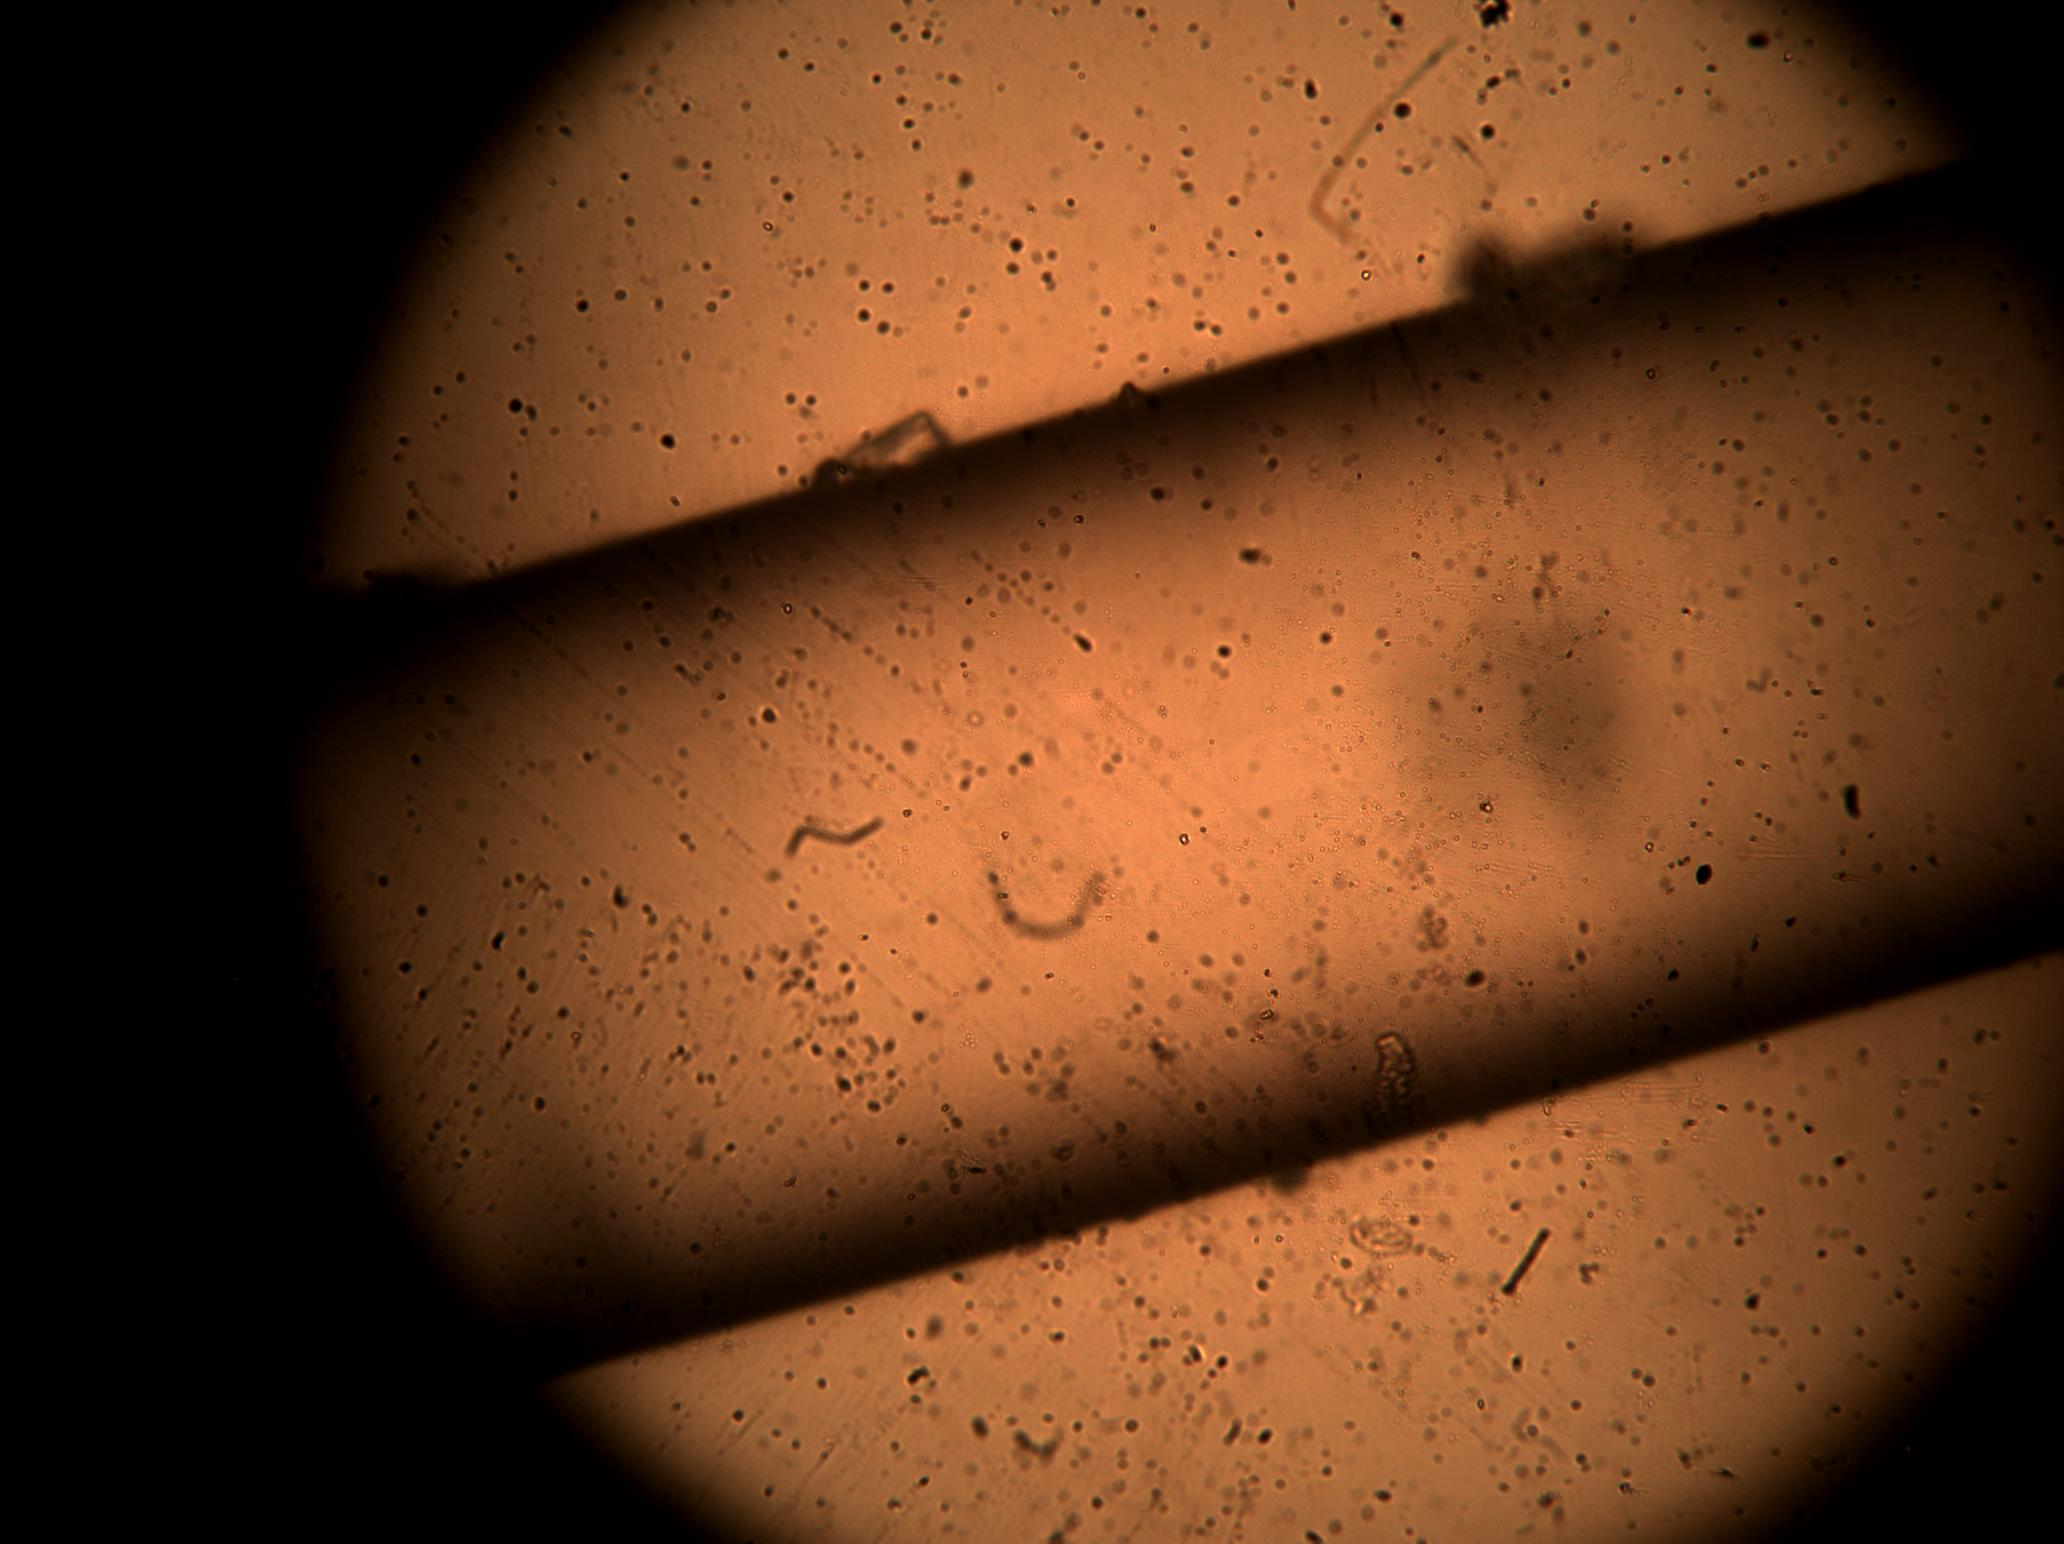
\includegraphics[width=7cm]{afbeeldingen/size/gf.jpg}
    \captionsetup{font=small, justification = centering}
    \caption{Image used to find $d_{gf}$.}
    \label{fig_gf}
\end{figure}

\newpage

The values that have been found for $a$, $b$, $A$ and the corresponding errors are presented in table \ref{table_zetmeel}.

\begin{table}[h!]
\centering
\captionsetup{font=small, justification = centering}
  \caption{Results of measurements of $a$ and $b$ for 30 starch particles. It was estimated that $u(a) =u(b) = 2 \: pixels$. The values for $A$ and $u(A)$ follow from respectfully equation \ref{eq_ellipse area} and \ref{eq_u_ellipse_area}. The particles corresponding to each number can be seen in figures \ref{fig_zetmeel_1} to \ref{fig_zetmeel_6}.}

\begin{tabular}{|l|l|l|l|l|} \hline
Particle number & $a \: (\# pixels)$ & $b \:  (\# pixels)$ & $A \: \cdot 10^{-10} \; (m^2)$ & $u(A) \: \cdot 10^{-12} \; (m^2)$ \\ \hline
1               & 84                 & 76                 & 1.28                           & 5                                 \\
2               & 83                 & 75                 & 1.25                           & 5                                 \\
3               & 85                 & 77                 & 1.32                           & 5                                 \\
4               & 72                 & 67                 & 0.97                           & 4                                 \\
5               & 97                 & 94                 & 1.83                           & 6                                 \\
6               & 58                 & 58                 & 0.68                           & 3                                 \\
7               & 70                 & 66                 & 0.93                           & 4                                 \\
8               & 105                & 95                 & 2.01                           & 6                                 \\
9               & 92                 & 90                 & 1.67                           & 5                                 \\
10              & 84                 & 82                 & 1.39                           & 5                                 \\
11              & 115                & 115                & 2.66                           & 7                                 \\
12              & 146                & 128                & 3.76                           & 8                                 \\
13              & 119                & 110                & 2.63                           & 7                                 \\
14              & 76                 & 75                 & 1.15                           & 4                                 \\
15              & 112                & 108                & 2.43                           & 6                                 \\
16              & 127                & 125                & 3.19                           & 7                                 \\
17              & 99                 & 90                 & 1.79                           & 6                                 \\
18              & 84                 & 81                 & 1.37                           & 5                                 \\
19              & 135                & 123                & 3.34                           & 8                                 \\
20              & 80                 & 78                 & 1.26                           & 5                                 \\
21              & 86                 & 84                 & 1.45                           & 5                                 \\
22              & 112                & 106                & 2.39                           & 6                                 \\
23              & 105                & 103                & 2.18                           & 6                                 \\
24              & 74                 & 72                 & 1.07                           & 4                                 \\
25              & 117                & 116                & 2.73                           & 7                                 \\
26              & 90                 & 83                 & 1.50                           & 5                                 \\
27              & 100                & 91                 & 1.83                           & 6                                 \\
28              & 117                & 104                & 2.45                           & 6                                 \\
29              & 100                & 97                 & 1.95                           & 6                                 \\
30              & 99                 & 92                 & 1.83                           & 6\\ \hline
\end{tabular}
\label{table_zetmeel}
\end{table}

\newpage

The images that were used to find the data in table \ref{table_zetmeel} can been seen in figure \ref{fig_zetmeel}

\begin{figure}[h!]
	
    \begin{subfigure}[b]{0.475\textwidth}
        \centering
        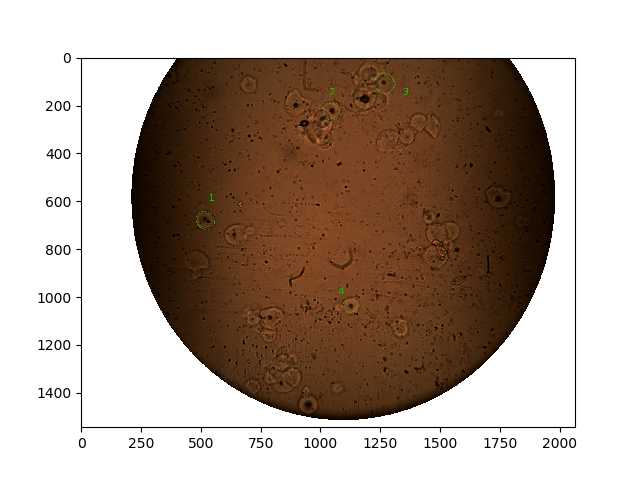
\includegraphics[width=\textwidth, frame]{afbeeldingen/size/zetmeel/zetmeel_1.png}
        \caption{Best ellipse fits for starch particles 1 to 4.}   
        \label{fig_zetmeel_1}
    \end{subfigure}
    \hspace*{\fill}
    \begin{subfigure}[b]{0.475\textwidth}
        \centering
        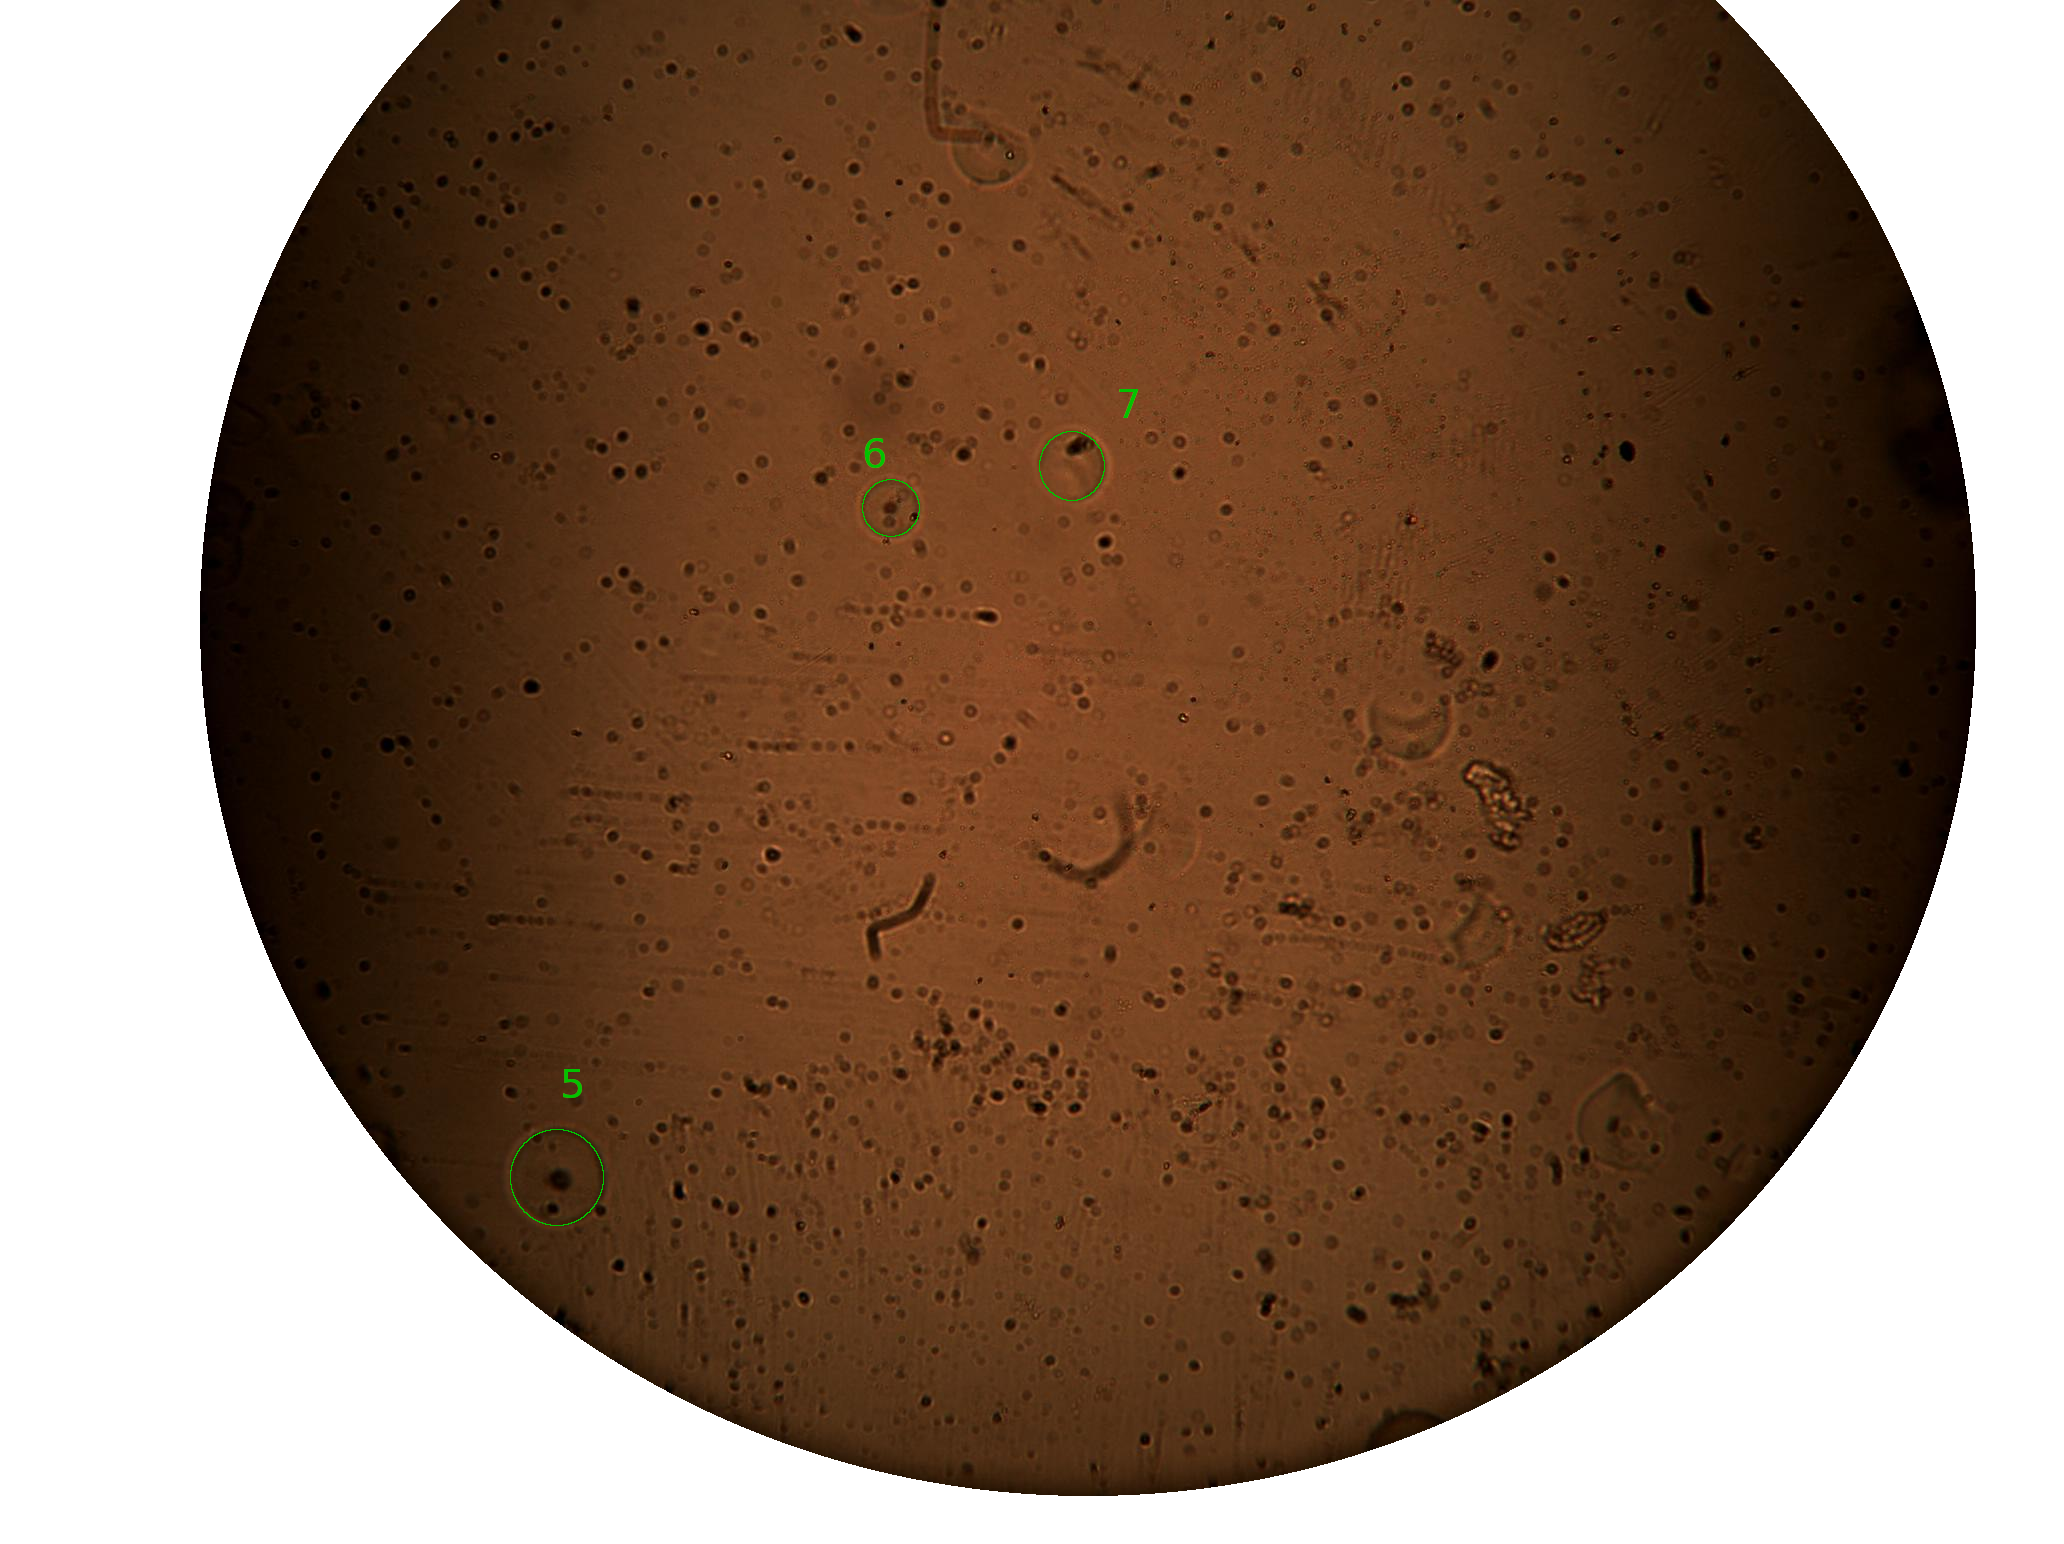
\includegraphics[width=\textwidth, frame]{afbeeldingen/size/zetmeel/zetmeel_2.png}
        \caption{Best ellipse fits for starch particles 5 to 7.}   
        \label{fig_zetmeel_2}
    \end{subfigure}
    
    \medskip
    \begin{subfigure}[b]{0.475\textwidth}
        \centering
        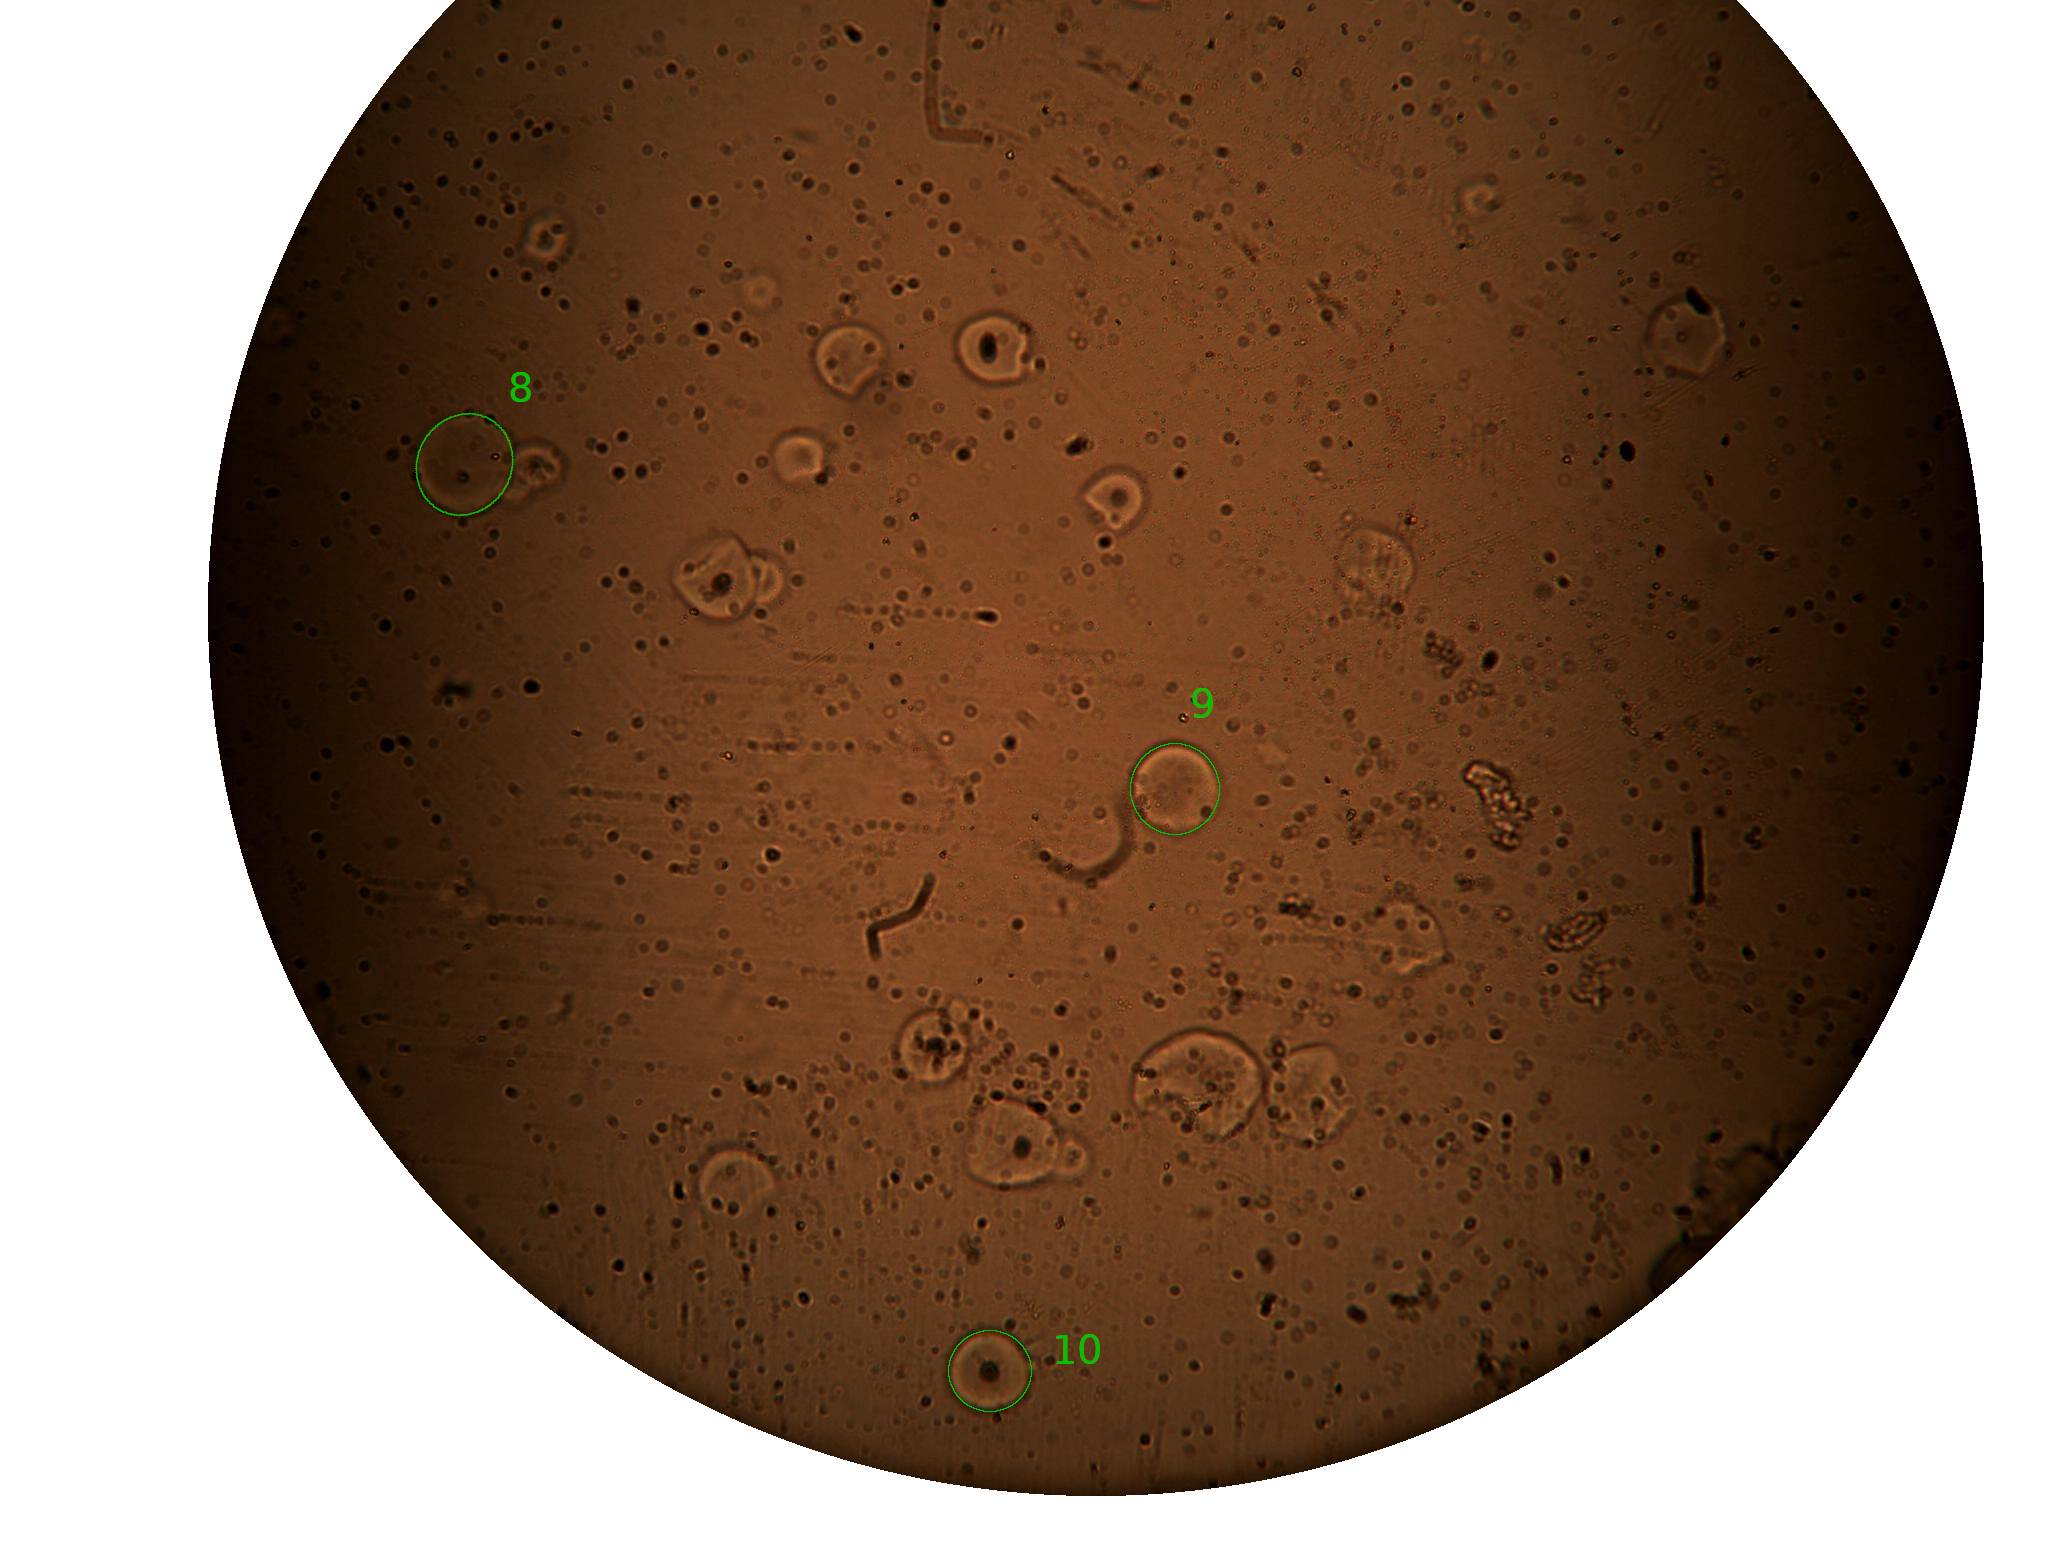
\includegraphics[width=\textwidth, frame]{afbeeldingen/size/zetmeel/zetmeel_3.png}
        \caption{Best ellipse fits for starch particles 8 to 10.}   
        \label{fig_zetmeel_3}
    \end{subfigure}
    \hspace*{\fill}
    \begin{subfigure}[b]{0.475\textwidth}
        \centering
        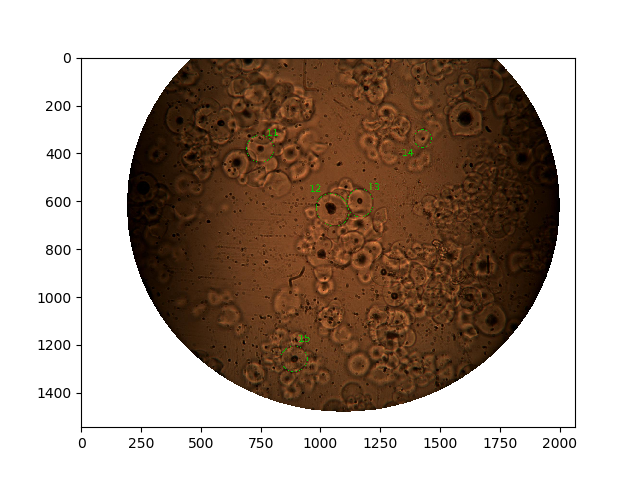
\includegraphics[width=\textwidth, frame]{afbeeldingen/size/zetmeel/zetmeel_4.png}
        \caption{Best ellipse fits for starch particles 11 to 15.}   
        \label{fig_zetmeel_4}
    \end{subfigure}
    
    \medskip
    \begin{subfigure}[b]{0.475\textwidth}
        \centering
        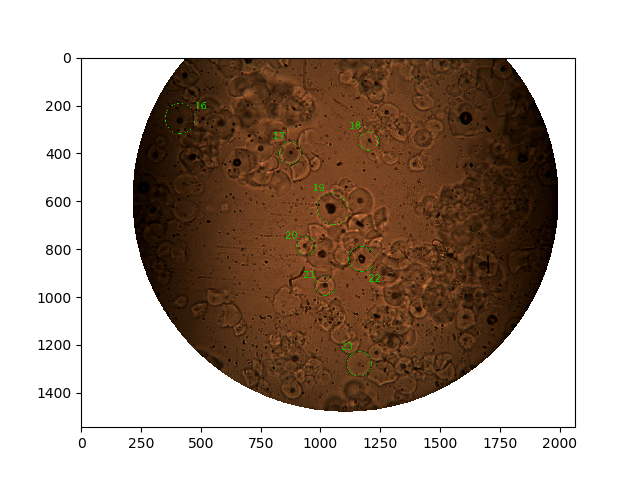
\includegraphics[width=\textwidth, frame]{afbeeldingen/size/zetmeel/zetmeel_5.png}
        \caption{Best ellipse fits for starch particles 16 to 23.}   
        \label{fig_zetmeel_5}
    \end{subfigure}
    \hspace*{\fill}
    \begin{subfigure}[b]{0.475\textwidth}
        \centering
        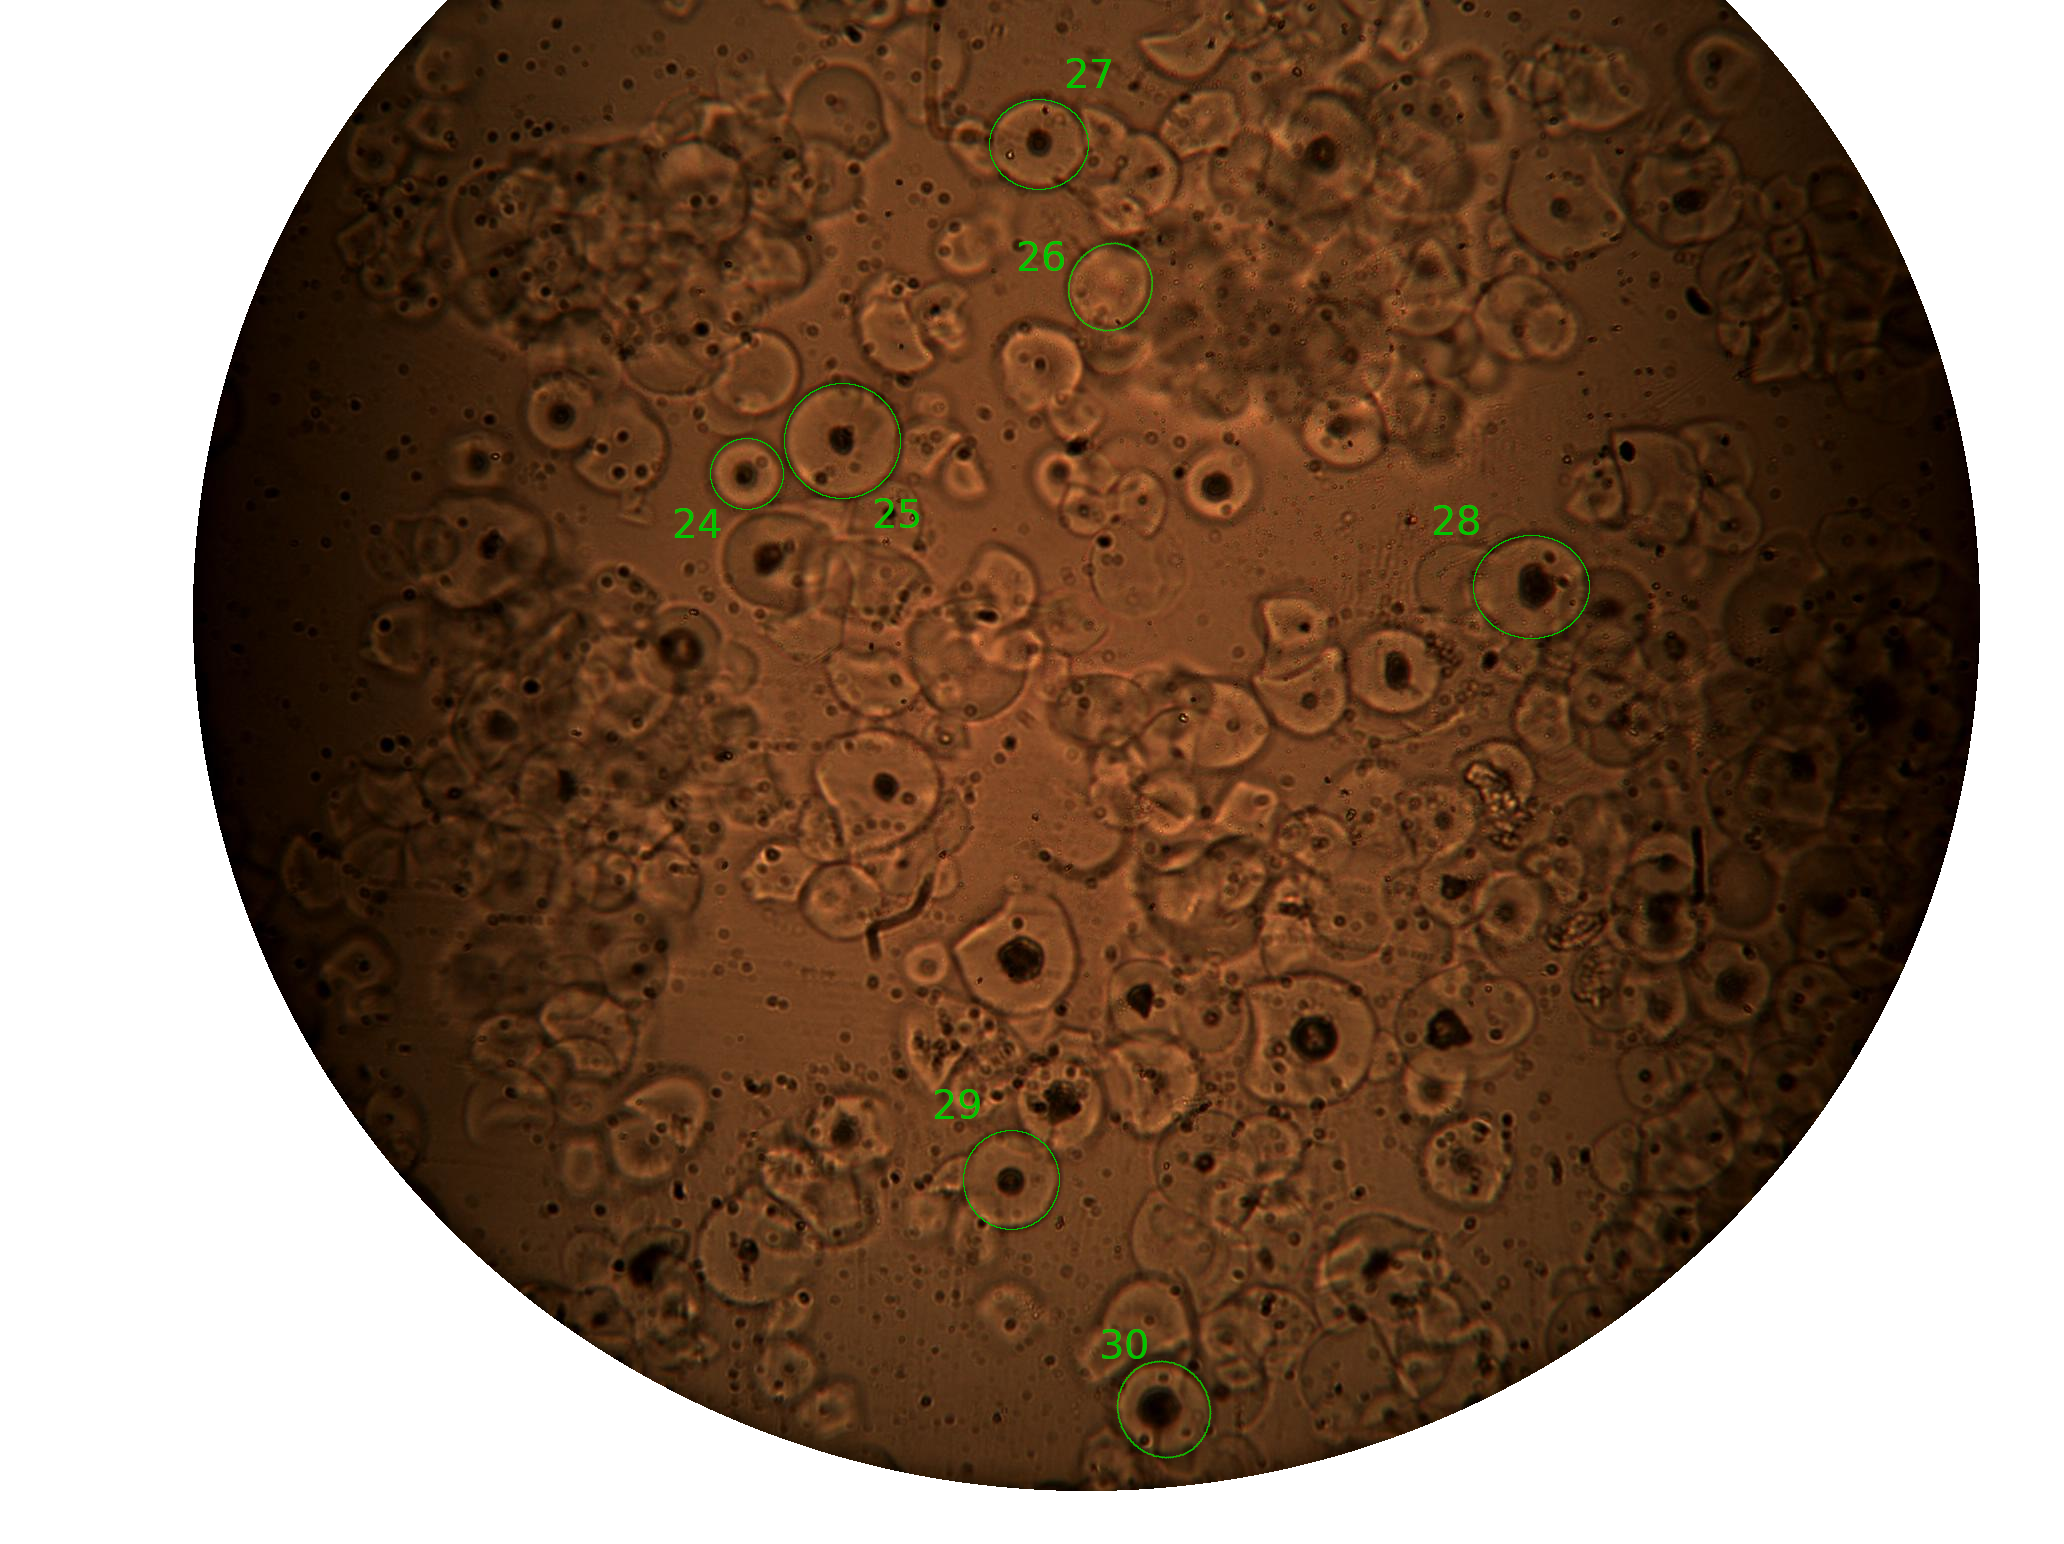
\includegraphics[width=\textwidth, frame]{afbeeldingen/size/zetmeel/zetmeel_6.png}
        \caption{Best ellipse fits for starch particles 24 to 30.}   
        \label{fig_zetmeel_6}
    \end{subfigure}
    
    \caption{Set of images used to find best ellipse fits for 30 starch particles. The green ellipses represent the best fit.} 
	\label{fig_zetmeel}
\end{figure}
